\documentclass{sig-alternate}


\usepackage{algorithm}
\usepackage{algorithmic}
\usepackage{amsmath}
\usepackage{amssymb}
\usepackage{array}
\usepackage{booktabs} 
\usepackage{cases}
\usepackage{enumitem}
\usepackage{epstopdf}
\usepackage{graphicx}
\usepackage{listings}
\lstset{
  basicstyle=\ttfamily,
  columns=fullflexible,
  frame=single,
  breaklines=true,
  postbreak=\mbox{\textcolor{red}{$\hookrightarrow$}\space},
}
\usepackage{longtable}
\usepackage{makecell}
\usepackage{multirow}
\usepackage{stfloats}
\usepackage{subeqnarray}
\usepackage{xcolor}
\usepackage{diagbox}

\lstset{
    escapeinside={(*}{*)}
}

%\usepackage{authblk}
\usepackage[caption=false,font=footnotesize]{subfig}

\newtheorem{problem}{Problem}

%\setcopyright{rightsretained}

% DOI
%\acmDOI{10.475/123_4}

% ISBN
%\acmISBN{123-4567-24-567/08/06}

%Conference
%\acmConference[MobiCom'18]{}{}{}
%\acmYear{2018}
%\copyrightyear{2018}

%\acmPrice{15.00}

%
\def\sharedaffiliation{%
\end{tabular}
\begin{tabular}{c}}
%

\newcommand{\sdn}{Malak}


\newcommand{\simpleTput}{80\%}    % overall throughput
\newcommand{\simpleLife}{20\%}    % lifetime increase using basic routing
\newcommand{\diagLife}{25\%}      % lifetime increase using diagnosis
\newcommand{\seleLife}{35\%}      % lifetime increase using selection algo.


\begin{document}

\title{{\sdn}: An Intelligent, High-performance and Resilient Software Defined Wireless Sensor Network System}
\author{}

%energy exhaustion


\maketitle

\begin{abstract}


A software defined network (SDN) enables  
many techniques (e.g., artificial intelligence, or AI) to be implemented easily, and in
turn these techniques greatly improve the performance and resilience of the SDN system.
Unfortunately, all the existing SDN systems in wireless sensor networks
are implemented in simulators, and there is no practical 
SDN implementation for wireless sensor networks.


In this paper, we present {\sdn}, the first practical SDN wireless sensor network system,
which achieves intelligence, high-performance and resilience simultaneously.
In {\sdn}, we utilize a set of unmanned aerial vehicles (UAVs) to serve as the SDN controllers. 
Sensor nodes communicate with UAVs when they are within one-hop communication ranges, 
greatly improving throughputs and reducing the sensor nodes' energy consumption. 
{\sdn} includes easy-to-use SDN interfaces and we have implemented five SDN applications, namely
routing, multi-task, network diagnosis, AI energy exhaustion prediction, and AI node selection.
{\sdn} is a ecosystem where all SDN applications run simultaneously to benefit each other.
Our evaluation shows that {\sdn}'s throughput is  {\simpleTput} higher than two 
notable traditional sensor network routing protocols.
%by using the basic {\sdn} routing algorithm. 
Meanwhile, the average lifetime of sensor nodes in {\sdn} is 
{\simpleLife} longer than these two protocols. 
%By running our AI energy prediction %and AI selection 
%application,  the nodes' lifetime in {\sdn} further improves  by {\totalLife}. %and {\seleLife}
All source code and results of {\sdn} are released on \emph{anonymous}.
%


%throughput improves by 1.2X compared to two notable traditional sensor network routing protocols.

%throughput    comparing with other provence,  still maintains initial throughput 
%when  


%!TEX encoding = UTF-8 Unicodestate-of-the-art

\end{abstract}

\section{Introduction}

Why we are SDN ?

Software defined network is able to support flexible network programmability 
by using programmable data plane and centralized network controller.

OpenFlow focus on wired networks.

Challenges and opportunities of SDN for WSN:

Challenges: Limited resources of WSN nodes:
\begin{itemize}
\item	energy
\item	processing
\item	memory
\item	communication
\end{itemize}

Opportunities: 
\begin{itemize}
\item	Improve resource reuse
\item	Implement node retasking 
\item	Node and network management
\item	Enable experiments with new protocols
\end{itemize}



Why and How we can implement AI ?

How we combine Ai with other applications?


AI 

AI systems have been improving, and new advances in machine intelligence are creating seamless interactions between people and digital sensor systems.

 In sensor systems, applications can be found for a variety of tasks, including selection of sensor inputs, interpreting signals, condition monitoring, fault diagnosis, machine and process control, machine design, process planning, production scheduling, and system configuring. Some examples of specific tasks undertaken by expert systems are:
* Assembly 
* Automatic programming 
* Controlling intelligent complex vehicles  
* Planning inspection 
* Predicting risk of disease 
* Selecting tools and machining strategies 
* Sequence planning 
* Controlling plant growth. 

.



The tools and methods described have minimal computation complexity and can be implemented on small assembly lines, single robots, or systems with low-capability microcontrollers. These novel approaches proposed use ambient intelligence and the mixing of different AI tools in an effort to use the best of each technology. The concepts are generically applicable across many processes.


minimum energy, data loss, reliability, robustness, etc., in place during the design and operation of wireless sensor networks

a specific set of protocols for medium access, localization and positioning, time synchronization, topology control, security and routing are identified based on the current configuration of the network, the requirements of the application and the topology of their deployment.
\section{Related work}

\subsection{Software Defined Wireless Sensor Networks}


Existing SDN for WSN:
\begin{itemize}
\item	Flow-Sensor
\item	Sensor OpenFlow
\item	SDWN
\item	TinySDN
\item	SDN-WISE
\end{itemize}
All of these are evaluated by simulations


Flow-Sensor [MahmudandRahmani2011], 
Sensor OpenFlow [Luoetal.2012] 
SDWN [Costanzo et al. 2012]
TinySDN [de Oliveira et al. 2014]
SDN-WISE [Galluccio et al. 2015]



Sensor SDN
Flow Sensor
The previous idea presented in paper [Flow-Sensor, 2011] addresses reliability in the sensor networks through exploiting the OpenFlow technology. Coming up with the concept of flow-sensor instead of typical sensor, they have successfully made it possible to communicate between controller, gateway and sensors. Besides that, they proved flow sensor more reliable since data packets, control packets and the sensor nodes themselves can be easily monitored, regulated and routed whenever required. Therefore, a robust routing and uninterruptable messages flow of sensors are achieved. The results described in this paper shows flow-sensor is able to display much better performance even for large networks.

SDWN
	The solution of supporting the SDN approach in LR-WPANS is first presented in [SDWN, 2012]. Given the gap that advantages of SDN and the proper ways to expand that to wireless network were not clear enough, the group analyzes the opportunities of SDN-related wireless network and illustrates the requirements should be considered to utilize SDN solution for wireless network. They made a good attempt to develop the SDWN protocol stack.

Sensor OpenFlow
	In the paper [sensor openflow], the group toke a radical, yet backward and peer compatible, approach to tackle the problems existing in WSN such as resource underutilization, counterproductive, rigidity to policy change and manage difficulty. They propose SD-WSN with a separation between data plane performing flow-based packet forwarding and control plane performing network control. The core part designed is Sensor OpenFlow(SOF), which gives a standard protocol for the communication between data and control part. Based on the whole architecture they gave, the underlying network becomes programmable by using SOF.

Tiny SDN
	TinySDN is a TinyOS-based SDN framework aims to address the problem that only single controller can be coupled to the sink. Besides, TinySDN is a hardware independent framework that comprises two parts: SDN-enable sensor node and SDN-controller node. In order to test the reliability of this framework, the authors done some experiments on COOJA. Through analyzing results concerning delay and memory footprint, they found it is feasible in communication provided by SDN paradigm.

SDN-WISE
	One solution for wireless sensor network is introduced in the paper[SDN-WISE], and the authors implement the prototype of this idea. Compared to other SDN solutions for wireless network, this solution successfully reduces the messages exchange needed between sensor node and controller. Besides, flexible APIs are provided by the authors, thus making the network much easier to program. Also, they done some experimental testbed, found that in a power limit hardware, the response delay is still very small, SDN-WISE shows its good performance in different operation conditions.

Sensor Select
	Redundant sensor network always contains nodes that generating data stream with some overleap parts. Collected information can be useful to determine which sensors are active. The algorithms come up with in paper[SS] are called Spatially Regularized Streaming Sensor Selection(SRSSS). The authors not only consider the spatial information but also the historical obversion of the sensor network. They apply higher weights to nearby sensors and introduce a time-forgetting factor so that their approach can predict more accuracy and response much faster than others.




\subsection{Applications for Wireless Sensor Networks}

Routing
Low-power and lossy network consist of devices whose processing, memory and energy are both constrained. Hence, traditional protocols can’t be used there. However, RPL is one of the standards for ipv6 routing in LLN. It builds the topology like a tree, performing DAO, DIO, ACK to generate a directed acyclic graph from one or more root to the leaf nodes. The experiments done in the paper [Low-Power Wireless IPv6 Routing with ContikiRPL] shows that Ipv6 routing with ContikiRPL is both lightweight and power-efficient.
 
Diagnosis
	Previous diagnosis algorithms share the same drawback that their process of gathering information is static and the reports sent to be analysis is not intermediate enough. Directional Diagnosis is an online diagnosis approach to dynamically recognize the most useful information according to an engine designed in the approach. Besides, the diagnosis process only focuses on the problematic area, so that it can produce a more accuracy prediction. To be specify, the whole approach consist of four main parts: Node Tracing, Trace Collection, Inference Model and Incremental Probing. The node tracing algorithms dynamically reconstruct topical topology and derive inner dependencies. Based on the data information collected, inference model can guide the next probe by Incremental Probing applying Belief network. The experiments done show the diagnosis result is efficient and in real time.

AI sensor
	The application of sensors often relays on the filed like sensor select, data prediction combining with AI algorithms. In order to select the subset of nodes to be active, related study give a way to dynamically response to the change of sensor network based on the historical information, the new sensor node has a different time factor from the old node when construct the predict network. Besides, the position of nodes may be highly used to reduce the weight of nearby nodes in a predict network. As for data prediction, on the one hand, the energy consuming information can be collected. Previous work on diagnosis, for example, only performs diagnosis when sensor almost run out of energy. On the other hand, the original data about temperature, humidity, light intensity is a reliable resources for prediction in time series. 

Multitask
	One single sensor node may shoulder several tasks. To achieve power saving, when a task performed, we need to choose which sensor to be active and which to be inactive. Nowadays, work aims to design an energy-efficient sensor management strategy tends to develop their method in three ways: choose the proper subset of nodes to be active, which sensors to assign the task and the sampling rate on one node when performing task. Related study has found an efficient online algorithm considering sensor activation and task mapping to deal with dynamic events during runtimes of SDSNS.

\section{Architecture}

The architecture of the UAV based SDN system for wireless sensor networks.

\begin{figure}[htbp]
	\centering
	\includegraphics[width=3.5in]{./Figure/Architecture}
	\caption{Architecture of the system.}
	\label{Architecture}
\end{figure}



\begin{table*}[htbp]
	\caption{System API}
	\label{API}
	\centering
	\scalebox{0.9}{
	\begin{tabular}{|l|l|}
		\hline
		\makecell[tc]{\textbf{Structure \&\& Function}} & \makecell[tc]{\textbf{Description}} \\
		\hline
		\multicolumn{2}{|c|}{\textbf{Sensor Control Interface}}\\
		\hline
		struct node & Sensor node structure\\
		\hline
		struct nodeset & A set of sensor nodes \\
		\hline
		struct neighbor\_list & Neighbor infomation \\
		\hline
		struct energy\_item & Energy statistic information \\
		\hline
		struct routing\_table & Routing table \\
		\hline
		struct duty\_cycle\_table & Duty cycle control table \\
		\hline
		struct sensor\_enable\_table & All the nodes's states. Node state: \{on,off\} \\
		\hline
		switch\_node(node,state) & Turn on or turn off the node \\
		\hline
		get\_node\_info(node) & Get node's information, including  node's position, duty cycle, power, etc.\\
		\hline
		set\_node\_attr(node,attrTag,value) & Set node attribute, including  duty cycle, radio strength, etc. \\
		\hline
		get\_neighborlist(node) & Get the neighbor list of a node \\
		\hline
		\multicolumn{2}{|c|}{\textbf{UAV Application Interface}}\\
		\hline
		\multicolumn{2}{|c|}{\textbf{Routing}}\\
		\hline
		get\_topology() & Get the topology of the network\\
		\hline
		get\_route(node) & Get the routing table of a node \\
		\hline
		set\_route(route\_table,node) & Set the routing table of a node \\
		\hline
		\multicolumn{2}{|c|}{\textbf{AI Node selection}}\\
		\hline
		nodeset simple\_selection(nodeset) & Select sensor set by location information\\
		\hline
		nodeset SRSSS\_selection(dataset) & Select sensor set by AI algorithm based on sensing data\\
		\hline
		\multicolumn{2}{|c|}{\textbf{AI Energy Prediction}}\\
		\hline
		model\_selsct(modeltype) & Select an AI model\\
		\hline
		model.train(dataset,ratio) & Train an AI model with learning ratio on the data set\\
		\hline
		model.test(dataset) & Test the AI model on the data set\\
		\hline
		model.predict(node) & Do the energy prediction for a node \\
		\hline
		\multicolumn{2}{|c|}{\textbf{Multi-tasks}}\\
		\hline
		create\_scheduler() & Create a task scheduler \\
		\hline
		scheduler.create\_buffer() & Create a task buffer \\
		\hline
		scheduler.task\_buffer\_add(task,nodenum) & Add a new task to task buffer \\
		\hline
		scheduler.task\_schedule() & Schedule the tasks in the buffer\\
		\hline
		\multicolumn{2}{|c|}{\textbf{Diagnosis}}\\
		\hline
		detect() & Detect problematic region with probes \\
		\hline
		get\_topical\_topology(nodeset) & Construct topical topology\\
		\hline
		diagnose\_network(topology,nodeset) & Diagnose the failure nodes or lossy links\\
		\hline
	\end{tabular}
	}
\end{table*}

\begin{lstlisting}[language={[ANSI]C},label=update,caption={An example of deploy routing algorithm},keywordstyle=\color{blue!70},showstringspaces=false, commentstyle=\color{red!50!green!80!blue!70},frame=single,captionpos=t, rulesepcolor=\color{red!20!green!20!blue!20}]
topology = get_topology();
//calculate routetable for each node 
//based on topology 
for(node in nodeset){
	node.routetable = 
		calculate_route(topology);
}
//set route for each node
for(node in nodeset){
	UAV fly to node;
	for(route in node.routeTable) 
  		set_route(route);
}

\end{lstlisting}


%\section{Network construction}

\subsection{Sensor selection}
ssss
Physical topology :  uniform distribution (Density ρ).

Sensor selection algorithm:
\begin{itemize}
\item[1)] A simple cluster algorithm: threshold δ -The distance between sensors \&\& the overlapping of sensing area \&\& the similar neighbor list. 
\item[2)] SRSSS Algorithm (AAAI-16) - trained by an AI model based on the collected data. 
\end{itemize}

Output : Redundant nodes

\subsection{Topology Mapping}

Redundant nodes are mapped to a virtual node. 
They can awaken each other according to their  residual energy. 
When:    
$$
\begin{aligned}                        
ResidualEnergy(i) \leq \xi \cdot ResidualEnergy(j) & &   {turn~node~i~to~node~j}\\
\end{aligned}
$$

These virtual nodes are called critical nodes in the logical topology while other nodes are called ordinary nodes.

\subsection{Logical routing}

Critical nodes first (CNF) algorithm
\section{Applications}

\subsection{Overview}

Traditional applications can not achieve complicated and efficient goals due 
to the limited processing power and memory space of sensors.

In {\sdn}, applications for wireless sensor networks are inspired by 
greater potential with the UAV based SDN controller. The central controller
helps sensors execute complex calculations such as AI model training, as well 
as store global information. Besides, UAVs have flexible features and can deploy 
tasks to sensors by one-hop communication directly. Thus it enables the sensor network
to achieve much more intelligent applications.

In {\sdn}, applications can be found for a variety of purposes, including routing, AI node selection,
Ai energy prediction, multi-tasks and network diagnosis. We design all these applications and provide 
easy-to-use interfaces to users as in Table \ref{API}.



\subsection{Routing}

\begin{table}[htbp]
	\caption{Flow Table}
	\label{FT}
	\centering
	\scalebox{0.9}{
	\begin{tabular}{|l|l|l|}
		\hline
		Header Fields & Counters & Actions \\
		\hline
		\end{tabular}
	}
\end{table}

\begin{table}[htbp]
	\caption{Header Fields}
	\label{HF}
	\centering
	\scalebox{0.9}{
	\begin{tabular}{|l|l|l|l|l|}
		\hline
		Ingress port & Ether Source & Ether Dst &IP src & IP dst \\
		\hline
		\end{tabular}
	}
\end{table}

Actions:
\begin{itemize}
\item	Forward
\item	Drop
\item	Report
\end{itemize}

\subsection{AI Node Selection}

\subsubsection{Motivation}

\subsubsection{Design}

Greedy selection algorithm.

\begin{algorithm}
\caption{Greedy Selection Algorithm}
\label{Greedy}
\begin{algorithmic}[1]
\STATE Input: Sensor set $N$, Selected set $M$, Target area $\Omega$, Covering area $\Phi$;
\STATE Initialize : $M = \emptyset$, $\Phi = \emptyset$
\WHILE {$M \neq N$}
    \IF{$\Phi = \Omega $}
        \STATE break; $\backslash$$\backslash$ selected set has been found
    \ENDIF
    \IF{$\forall n_i \in (N-M) : range(n_i) \subset \Phi$}
    	 \STATE break;$\backslash$$\backslash$ Cannot cover the target area;
    \ENDIF
    \STATE Find $n_i : argmax(\Phi \cap range(n))$, $n_i \in (N-M)$;
    \STATE $\Phi = \Phi \cup {n_i}$
\ENDWHILE
\STATE Output: $M$;
\end{algorithmic}
\end{algorithm}

SRSSS AI algorithm selection.

\begin{figure}[htbp]
	\centering
	\includegraphics[width=2in]{Figure/OF}
	\caption{Objective function.}
	\label{system}
\end{figure}


**************

AI helps creating smarter sensor systems.

AI systems have been improving, and new advances in machine intelligence are creating seamless interactions between people and digital sensor systems.

 In sensor systems, applications can be found for a variety of tasks, including selection of sensor inputs, interpreting signals, condition monitoring, fault diagnosis, machine and process control, machine design, process planning, production scheduling, and system configuring. Some examples of specific tasks undertaken by expert systems are:
* Assembly 
* Automatic programming 
* Controlling intelligent complex vehicles  
* Planning inspection 
* Predicting risk of disease 
* Selecting tools and machining strategies 
* Sequence planning 
* Controlling plant growth. 

AI can increase effective communication, reduce mistakes, minimize errors, and extend sensor life.



The tools and methods described have minimal computation complexity and can be implemented on small assembly lines, single robots, or systems with low-capability microcontrollers. These novel approaches proposed use ambient intelligence and the mixing of different AI tools in an effort to use the best of each technology. The concepts are generically applicable across many processes.


minimum energy, data loss, reliability, robustness, etc., in place during the design and operation of wireless sensor networks

a specific set of protocols for medium access, localization and positioning, time synchronization, topology control, security and routing are identified based on the current configuration of the network, the requirements of the application and the topology of their deployment.

\subsection{AI Energy Prediction}

\subsubsection{Motivation}

\subsubsection{Design}

\subsection{Multi-tasks}

\subsubsection{Motivation}

Wireless sensor networks (WSN)  generally comprise of a group of 
spatially dispersed sensors. In a wireless sensor network, 
sensor nodes are equipped with various 
types of sensors monitoring and recording 
environmental conditions like temperature, sound, sunlight,
humidity, etc.

A given sensing task involves multiple sensors to 
achieve a certain quality-of-sensing.
Generally, an efficient task scheduling for the nodes is that nodes 
are able to perform multiple tasks simultaneously. 
For example, sensors deployed in a grove are assigned tasks to collect
sunlight, temperature and humidity data and these tasks require different 
number of  nodes with respective sensing range, rate and duration.
However, traditional sensor networks are not suitable to conduct this 
multi-tasks due to the limitations of computation complexity for task 
arrangement of each node.

In our {\sdn} system, we implement the multi-tasks application 
with the help of the central controller. The SDN controller
maintains programmable task scheduling and management
modules while sensor nodes are loaded with interfaces to
receive task control instructions.     

\subsubsection{Design}

A deployed wireless sensor networks are usually assigned  


A sensor node may have different sensing ranges for different tasks.


There are several practical requirements.

Different tasks have different requirements, including time, sensing range, sensing ratio, etc.

For example tasks like sunlight collection only need to be carried out during the daytime.

Our system provide a task scheduling to 

Sensors are usually assigned multi-tasks.

Sensors are assigned tasks to monitor a specific area.

Different tasks have different requirements, including time, density, etc.

\begin{itemize}
\item[nodeset] kk
\item[sensing rate] energy
\item[sensing range] processing
\item[sensing duration] memory
\end{itemize}

Task scheduler do the arrangement. 

Task buffer.

Task queue.

Scheduling table.

...

\subsection{Network Diagnosis}

Diagnose the network.

\section{Implementation}
\label{Imp}

We run modified contiki-ng, a system for next generation IoT (Internet of
Things), on data plane. We modify the network layer of contiki-ng, and abstract
data plane interface to separate network control functions from data plane. 
The details are described as follows.

\textbf{Neighbor Discovery.} After deployment, nodes frist start IPv6 neighbor
discovery protocol to find the nodes which can be reached within one hop, and
then save the neighbor information to neighbor table and wait for UAV arriving
to gather the topology information. Every neighbor's information consists of the
neighbor's IP and RSSI. 

\textbf{Packet forwarding.} The nodes get routing table from UAV through
northbound interface. When a node receive a data packet from other nodes, it
just sends it to the next hop node according the routing table.

\textbf{Data sampling.} Nodes read task table received from UAV to decide when
to wake up sensors to make sure that they cost minimal energy to get the same
quality data. 

\textbf{UAV.} We run our UAV flight controller on ROS (Robot Operating System)
and use MySQL as our SDN database. UAV gathers topology from each node and save
it into database, so that users can easily read the whole network data from
database. For the same reason, after a user gets routing algorithm results and
saves it into database via northbound interface, our control plane will
automatically divides the whole network routing results into individual node's
routing table, and then sends it to specific nodes.

\begin{figure}[htbp]
	\centering
	\includegraphics[width=.85\columnwidth]{Figure/topology}
	\vspace{-0.1in}
	\caption{Network topology}
	\label{topology}
	\vspace{-0.1in}
\end{figure}

Based on our software framework, we use DJI M100 UAV with Intel NUC as airborne
computer, and adapt 250 TI CC2650 SensorTag to build our testbed. According to
our UAV gathered topology, we draw Figure~\ref{topology}, the blue lines
represent the connection between cluster members with cluster headers, and the
red lines donate the route between cluster headers deployed by UAV.

\section{Evaluation}
\label{Eva}

In this section, we describle our performance evaluation in simulation and
real-scene experiments. We distribute 130 TI SensorTag sensors in an about
$250~\times~250$ square meters area, with contiki-ng as its operating system. We
use different metrics for various applications and compare our works with other
state-of-the-art works.

\subsection{Routing}

\textbf{Packet loss ratio}

Packet loss ratio is defined as the proportion of the total data packets
recieved by data sink and the the total data packets sent by all nodes, and it
can be formulated as

\begin{equation}
	L = \frac{\sum_{i = 0}^{N}S_i}{R}
\end{equation}

where $L$ reprents the throughput, and $S_i$ and $R$ denotes the number of
packets sent by the $i$-th node and the number of packets recieved by data
sink, respectively.

\textbf{Total throughput}

\begin{figure}[htbp]
	\centering
	\includegraphics[width=.85\columnwidth]{Figure/throughput}
	\vspace{-0.1in}
	\caption{Routing throughput.
		\textnormal{
			The figure shows throughput corresponding to three kinds of Routing
			algorithms. Throughput can drop to zero when some key nodes are dead
			in the network.
		}}
	\label{fig:throughput}
\end{figure}

Throughput is defined as the the total data packets recieved by data sink, and it
measures the capability and scalability of a network.

Figure~\ref{fig:throughput} compares network throughput by deploying various
routing algorithms. As our {\sdn} uses OSPF, which finds the optimal path from
sensors to data sink, to caculate the route table, its throughput exceeds RPL
and LEACH. Besides, in {\sdn}, sensors' lifetime increases a lot more than
others, because all computation-intensive tasks are done by UAV and sensors do
not need to send packets to negotiate route path, which decrease the energy
consumption with no doubt.

\textbf{Fault tolerance}

Fault tolenrance is a significant metric to evaluate the performance of routing
algorithms. It measures the throughput with various number of node died.
Throughput can drop sharply if a node which most traffic passes by dies and can
be influenced only slightly by death of nodes which no traffic passes through.

We compare the impact caused by death of nodes using throughput between RPL and
{\sdn} and the results are shown in Figure~\ref{fig:fault_tolerance}. Throughput
can be low when the number of death is small, because we distribute the sensors
densely and the collision problem is severe. And the throughput grows as some
node died. But after some key nodes died, the throughput falls down quickly,
however, our {\sdn} still performs better than PRL.

\begin{figure}[htbp]
	\centering
	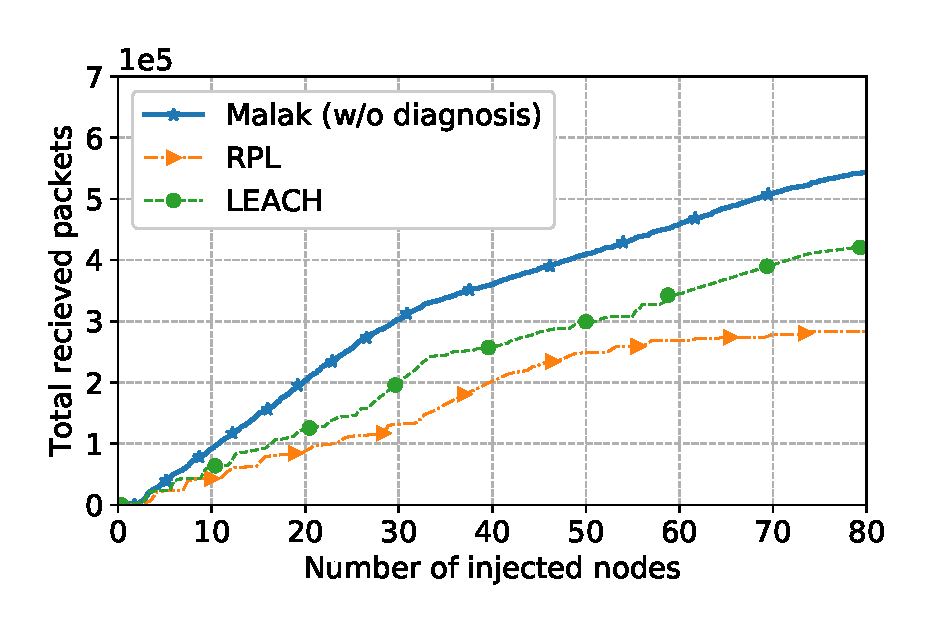
\includegraphics[width=.85\columnwidth]{Figure/fault_tolerance}
	\vspace{-0.1in}
	\caption{Fault tolerance
		\textnormal{
			RPL and {\sdn} are compared on fault tolerance, and {\sdn} perform
			slightly better than PRL.
		}}
	\label{fig:fault_tolerance}
\end{figure}

\textbf{Scalability}

\begin{figure}[htbp]
	\centering
	\includegraphics[width=.85\columnwidth]{Figure/scalability}
	\vspace{-0.1in}
	\caption{Scalability
		\textnormal{
			{\sdn} succeeds RPL in different network sizes.
		}}
	\label{fig:scalability}
\end{figure}

\subsection{Network Diagnosis}
\textbf{Robustness}

\subsection{AI Node Selection}
\textbf{Scalability}

\subsection{AI Energy Prediction}

We estimate sensor energy consumption by multipling different coefficients on
CPU running time and radio listening and transmitting time and summing them up.
The coefficients are proportional to the working current described in sensor's
DataSheet.

\textbf{Prediction accuracy}

\begin{figure}[htbp]
	\centering
	\subfloat[Energy prediction]{
		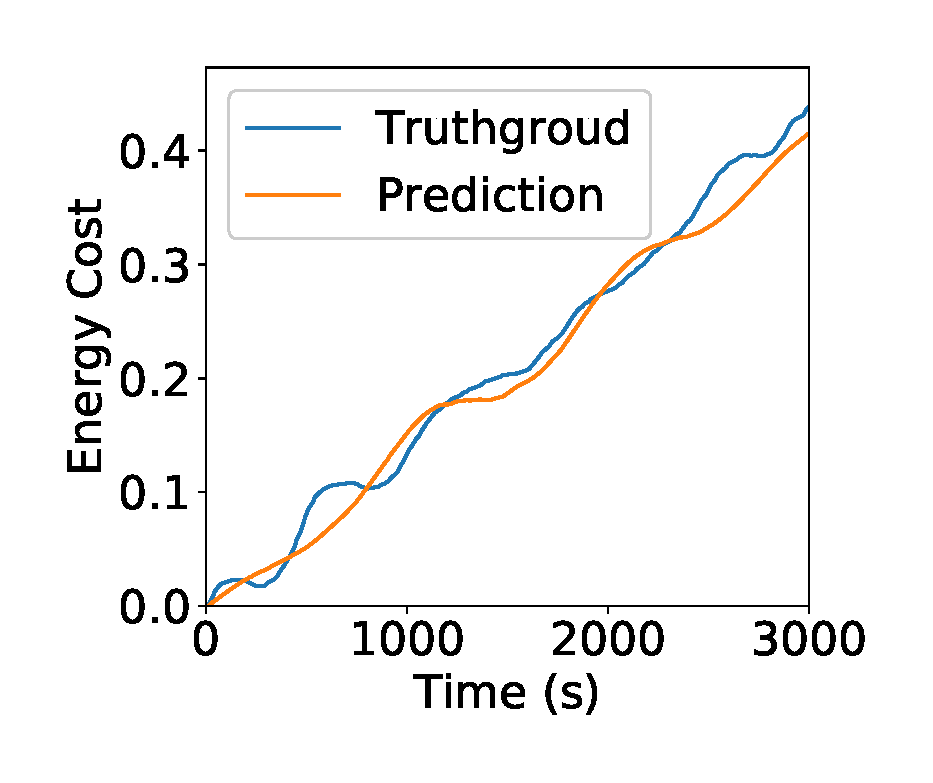
\includegraphics[width=.43\columnwidth]{Figure/energy_pred}
		\label{fig:energy_pred:a}
	}
	\hspace{0.3cm}
	\subfloat[Energy prediction error]{
		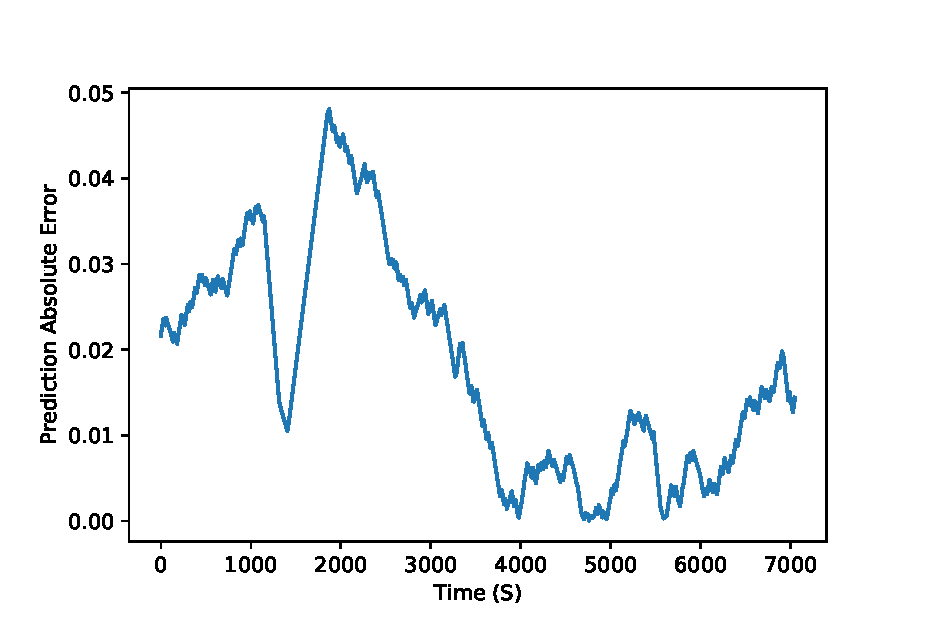
\includegraphics[width=.43\columnwidth]{Figure/energy_pred_err}
		\label{fig:energy_pred:b}
	}
	\vspace{-0.1in}
	\caption{Energy prediction
		\textnormal{
			We use regression method to predict energy consumption and the
			prediction result is consistent with the truthground.  The absolute
			error of energy prediction never exceeds 0.05 with normalized energy
			(i.e. the maximum energy of a sensor is 1).
		}
	}
	\label{fig:energy_pred}
\end{figure}

\subsection{Multi-tasks}
\textbf{Energy Performance}
\textbf{Scalability}
\begin{figure}[htbp]
	\centering
	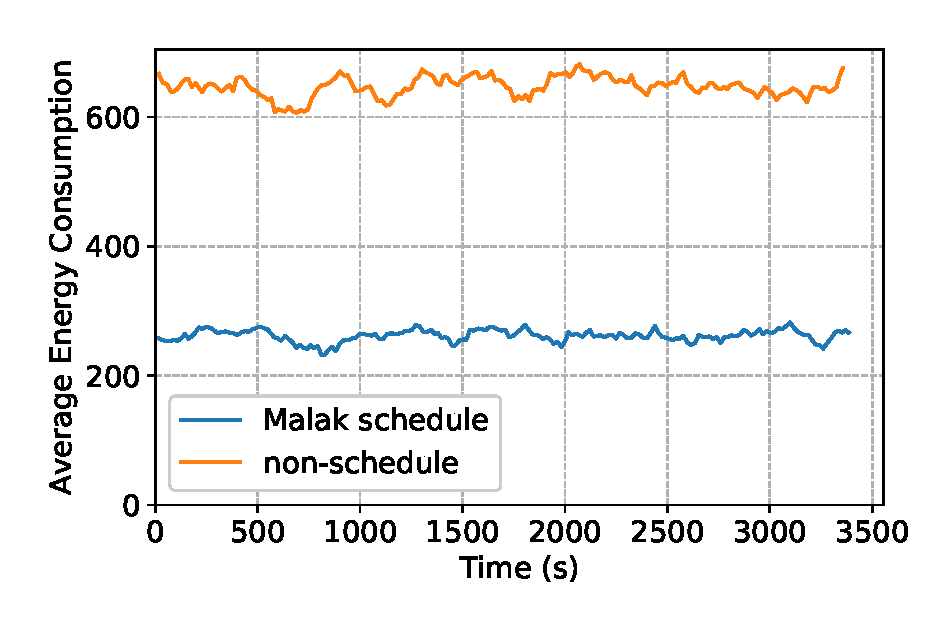
\includegraphics[width=.85\columnwidth]{Figure/multitask_energy}
	\vspace{-0.1in}
	\caption{Average energy consumption with and without multitask schedule
		\textnormal{When with multitask schedule, sensor consumes half of the energy
			comparing to when without multitask schedule.}}
	\label{fig:multitask_energy}
\end{figure}

\section{Conclusion}
\label{Con}

In this paper, we present {\sdn}, the first practical SDN 
wireless sensor network system,
which achieves intelligence, high-performance and 
resilience at the same time for general applications. 
Five typical applications: routing, network diagnosis, AI energy prediction, 
AI node selection and multi-task are realized in {\sdn}.
Our experiments show that {\sdn} 
improves the throughput by 80\% and prolongs the average lifetime of sensor nodes by 20\%. 
By running diagnosis and AI selection applications together, 
{\sdn} further increases the lifetime by 25\% and 35\% more, respectively.
All source code and results of Malak are ready to open source.


\bibliographystyle{acm}
\bibliography{Ref}

\end{document}
